\documentclass[ oneside,% the name of the author
                    author={Cassie Qing Tang},
                % the degree programme: BSc, MEng, MSci or MSc.
                    degree={BSc},
                % the dissertation    title (which cannot be blank)
                     title={An Automated Response System for Disrupting Online Pet Scamming \\ },
                % the dissertation subtitle (which can    be blank)
                    subtitle={ }]{dissertation}

\usepackage[english]{babel}
\usepackage[nottoc]{tocbibind}
\usepackage{graphicx}
\usepackage{subcaption}
\usepackage{float}
\usepackage[list=true]{subcaption}
\usepackage{caption}
\captionsetup[figure]{labelformat=empty} % This disables automatic labelling of graphics
\captionsetup[subfigure]{labelformat=empty} % This disables automatic labelling of graphics
\usepackage[utf8]{inputenc}
\usepackage{hyperref}



\begin{document}

\maketitle
\fronmatter

\chapter*{Abstract}
This project targets the growing threat of online pet scams by creating an automated system to waste scammers' time and resources, aiding in scam identification and prevention. Following extensive development and testing, a four-week experimental deployment against pet scammers unveiled and refined effective scam-baiting tactics.

\chapter*{Acknowledgements}
I would like to express my special thanks to my supervisor, Dr Matthew Edwards, for his help and guidance in this project.
\\
\\
I would also like to give my thanks to School of Engineering for inviting me into UoB Computer Science OpenAI Team, which reimburses me the cost of using the different APIs of OpenAI.
\\
\\
Sign up for GitHub Student Developer Pack provides me free access to many useful tools, involving \href{https://www.mailgun.com}{Maligun} and \href{https://www.name.com}{Name.com}. Appreciate the resources it provides!

\makedecl


\tableofcontents
\listoffigures
\listoftables

\chapter*{Ethics Statement}
An ethics application for this project was reviewed and approved by the faculty research ethics committee as application 17599.


\chapter*{Supporting Technologies}
I created my system based on an open-source GitHub repository from \url{https://github.com/an19352/scambaiter_back}. By extending and altering its code to fit my needs.
\\
\\
I integrated two GPT models, specifically GPT-3.5-turbo-0125 and GPT-4-0125-preview, into my system via their APIs to ensure the functionality of an automatic email reply feature. One necessary API key was acquired and configured using the resources available at \url{https://openai.com/}.
\\
\\
I applied my own domain name from \url{https://www.name.com/} in order to generate a large number of bait-email addresses.
\\
\\
I obtained a mailgun API key and build a mailbox server on \url{https://www.mailgun.com/}, which can support emails receiving, sending and tracking.

\chapter*{Notation and Acronyms}
\begin{quote}
\noindent
\begin{tabular}{lcl}
AFF                 &:     & Advance Fee Fraud    
 \\ 
HTTP/HTTPS          &:     & Hypertext Transfer Protocol/Hypertext Transfer Protocol Secure
 \\ 
HTML                &:     & Hypertext Markup Language
\\
XML                 &:     & Extensible Markup Language
\\
Regex               &:     & Regular Expression
\\
NLP                 &:     & Natural Language Processing
\\
SSL                 &:     & Secure Sockets Layer
\\
JSON                &:     & JavaScript Object Notation
\\
A*                  &:     & A-star
\\
GPT                 &:     & Generative Pre-Trained Transformer
\\
API/APIs            &:     & Application Programming Interface
\\
URL/url             &:     & Uniform Resource Locator
\\
UNIX/UNICS          &:     & UNiplexed Information Computing System
\\
DNS                 &:     & Domain Name System


\end{tabular}
\end{quote}


\mainmatter

\chapter{Introduction}
\label{chap:context}
In the definition of online scam, both advance fee and non-delivery frauds can be defined as a social engineering attack. The former is that fraudsters often promise their victims goods or more money in order to convince them to pay a fee upfront \cite{claude_toward_2014}. This scheme has been widely applied to lottery scams, inheritance scams, romance scams, etc. While the latter can be seen as a concrete realisation of the former that victims could never receive the goods even though they have sent the payment \cite{whittaker_understanding_2020}. In recent years, the happen of these two types of fraud have become increasingly frequently with the growing demand for online shopping and the development of logistics. According to the Internet Crime Report for 2019 \cite{noauthor_2019_nodate}, more than 60,000 Americans experienced non-delivery scams during the year, and another 14,607 Americans reported that they had been subjected to the AFF. The total amount of money involved in both reached nearly \$300 million. The newly released annual report for 2023 shows this amount has risen to \$450 million, even as the complaint count for the corresponding type of fraud has decreased \cite{noauthor_2023_nodate}. Simultaneously, the UK is also witnessing a similar rise in the prevalence of AFF with a substantial 549\% increase noted in March 2023 compared to three years prior \cite{stripe_crime_2023}. 
\\

Pet fraud is a typical scam involving AFF and non-delivery frauds. Scammers usually register a domain name at a very low cost to create their own e-commerce website. They attract consumers to purchase non-existent pets by placing a large number of online advertisements on social media such as Facebook and offering low prices \cite{price_resource_2020}. In order to quickly gain the trust of potential victims, scammers build seemingly legitimate websites. They prominently display on the homepage that they have joined some credible real organisations, or claim to be certified as top sellers of certain dog breeds, and display some fake consumer purchase reviews and services they have provided \cite{price_resource_2020}. In addition, most of the cute pet photos displayed on scam websites are sourced from other legitimate platforms \cite{better_business_bureau_bbb_2017}. Scammers attach the name, breed, age, and even fabricated stories about the pet alongside these stolen photos. People interested in owning pets are more likely to desire a purchase after seeing this information. They typically reach out to the scammers via the WhatsApp number, email address, or other contact details provided on the webpage. Alternatively, they may actively complete the contact form on the webpage.
\\

At this stage, most victims are almost trapped in pet scams. Scammers guide them towards private communication channels that are not supervised by regular e-commerce platforms, using pre-written scam templates to make false promises \cite{ipata_current_nodate}. Once trust is established, victims are asked to pay for pets using non-refundable payment methods like Western Union or MoneyGram, subsequently receiving a tracking number and a URL for a delivery website to track their orders \cite{price_resource_2020}. Unexpectedly, these websites are also controlled by the scammers. These 'pet orders' soon encounter various fictitious transportation and medical issues, resulting in continuous delays in the transaction \cite{price_resource_2020}. Capitalising on the victims' emotional investment, the scammers continuously request additional fees with new excuses until the victims realise they have been deceived. Consequently, the victims not only fail to receive the pets but also lose a significant amount of money. A report indicates that about two-thirds of scam victims in England and Wales have experienced mental health and sleep issues \cite{shaw_report_2024}, which is confirmed by Kanetria Hutcherson's experience \cite{better_business_bureau_bbb_2017}.
\\

The earlier data comes from a 2015 report by the Federal Trade Commission (FTC) in the United States, which recorded approximately 37,000 pet-related complaints \cite{better_business_bureau_bbb_2017}. The Better Business Bureau's (BBB) recent research indicates that, since 2017, pet scams have represented a quarter of online shopping fraud cases in the US, with the average yearly financial loss for victims continuing to rise \cite{better_business_bureau_bbb_2022}. Similar problems have been reported worldwide in recent years. For instance, Lloyds Bank in the UK noted a significant rise in pet scam complaints according to their released statistics \cite{lloyds_bank_fraudsters_2023}. Relevant research in Australia and Canada also reflects this trend \cite{better_business_bureau_bbb_2017}.
\\

Despite the above reports have revealed the mature modus operandi of pet scam gangs and their increasingly detrimental impact on society, pet scams have not received as much attention as other similar scams, such as romance scams. Current research and countermeasures are primarily focused on helping the public identify and prevent pet scams. This includes the reporting and searching functions provided by \href{https://www.ipata.org/pet-scams}{IPATA} and \href{www.petscams.com}{Petscams}, as well as \href{www.aa419.org}{AA419}, which operates a fake website database. Moreover, there are some technical development projects, such as the development of \textit{Scammed Posts Detector} \cite{norazman_development_2014} and the research of \textit{Automated classification of pet scam websites} \cite{mehmedov_automated_2021}. However, there is still a lack of targeted research that can effectively defend and disrupt such scams.
\\

This article will further investigate the field of pet scams. Based on the current operational mode of pet scams, an automatic response system that disrupts pet scams has been developed. This system is built on the basis of an expandable Scam-baiting Mail Server \cite{an19352_an19352scambaiter_back_2023}, aiming to contribute to the resistance and disruption of pet scams. As part of the project, multiple web crawlers will be built to extract and process various data. This includes the homepage URLs and the contact form pages on pet scam websites, as well as the implementation of automatic form filling. On the other hand, the system also needs the functionality to send and receive emails, as scammers will initiate email contact after receiving the form application. By building our own mail server and formulating various response strategies, we will conduct an one-month experimental interaction with pet scammers. After the experiment, relevant information and data will be integrated and analysed to determine the most effective response strategy. Finally, the project results are discussed comprehensively in terms of the success rate of script execution and the response rate of emails. The project execution intends to provide the public with powerful anti-pet scam strategies directly. Additionally, the automatic form-filling script can be paired with other advertisement scam detectors, such as the \textit{Scam Detection in Online Classified Advertisements} developed by Hamad Alsaleh \cite{alsaleh_scam_2017}. This can further assist more researchers and anti-fraud organisations in understanding and combating online fraud.
\\

Therefore, the specific objectives of this project can be summarised as the following key points:

\begin{itemize}
  \item Implement the automatic form-filling script and prove its feasibility through experimentation.
  \item Identify the best personality to disrupt pet scams, contributing to a safer online environment.
  \item Increase the understanding of pet scammers and their common methods used in emails, to help myself and others improve awareness of pet scams.
\end{itemize}


\chapter{Technical Background}
\section{Petscams.com}
The data for pet scam websites in this study was sourced from a volunteer organisation called \href{https://www.petscams.com}{Petscams}. This organisation operates a website, using the same domain name, to list fraudulent pet sales and shipping sites \cite{brady_fighting_2024}. \href{https://www.petscams.com}{Petscams.com} is an effective and free platform offering a range of security services to alert the public about the danger of those websites. These services include victim reporting and comment systems, fraudulent website analysis, verification, classification, and continuous article updates. They also provide access of these data to law enforcement agencies to better disrupt and combat scammer activities. Beyond that, they have been a valuable resource for other researchers. For instance, their victim report system significantly contributed to a pet scam case study published in 2020 \cite{whittaker_understanding_2020}.
\\

Figure 1 illustrates how articles on this website maintain consistent HTML structural features in the developer mode of the Chrome browser. It's clear to see each article is nested within an $<$article$>$ tag, which is part of the HTML5 semantic markup, used to define independent content modules on the website. Importantly, each article's title, which the suspected fraudulent domain information, is placed within the $<$h2$>$ tag. 
\\

Furthermore, as shown in Figure 2 and Figure 3, the page layout across different articles is also remarkably uniform. Each article segments the key points and introductory content, ensuring information is presented clearly. The breakdown of each scam website in the article consists of four main parts - identity, review credibility, legality, and recommended next steps - for in-depth description and analysis. This thoughtful design considerably assists victims and researchers, in quickly and fully understanding the workings of pet scams.
\begin{figure}[!htb]
    \centering
    % First bigger subfig
    \begin{subfigure}[b]{0.8\textwidth}
        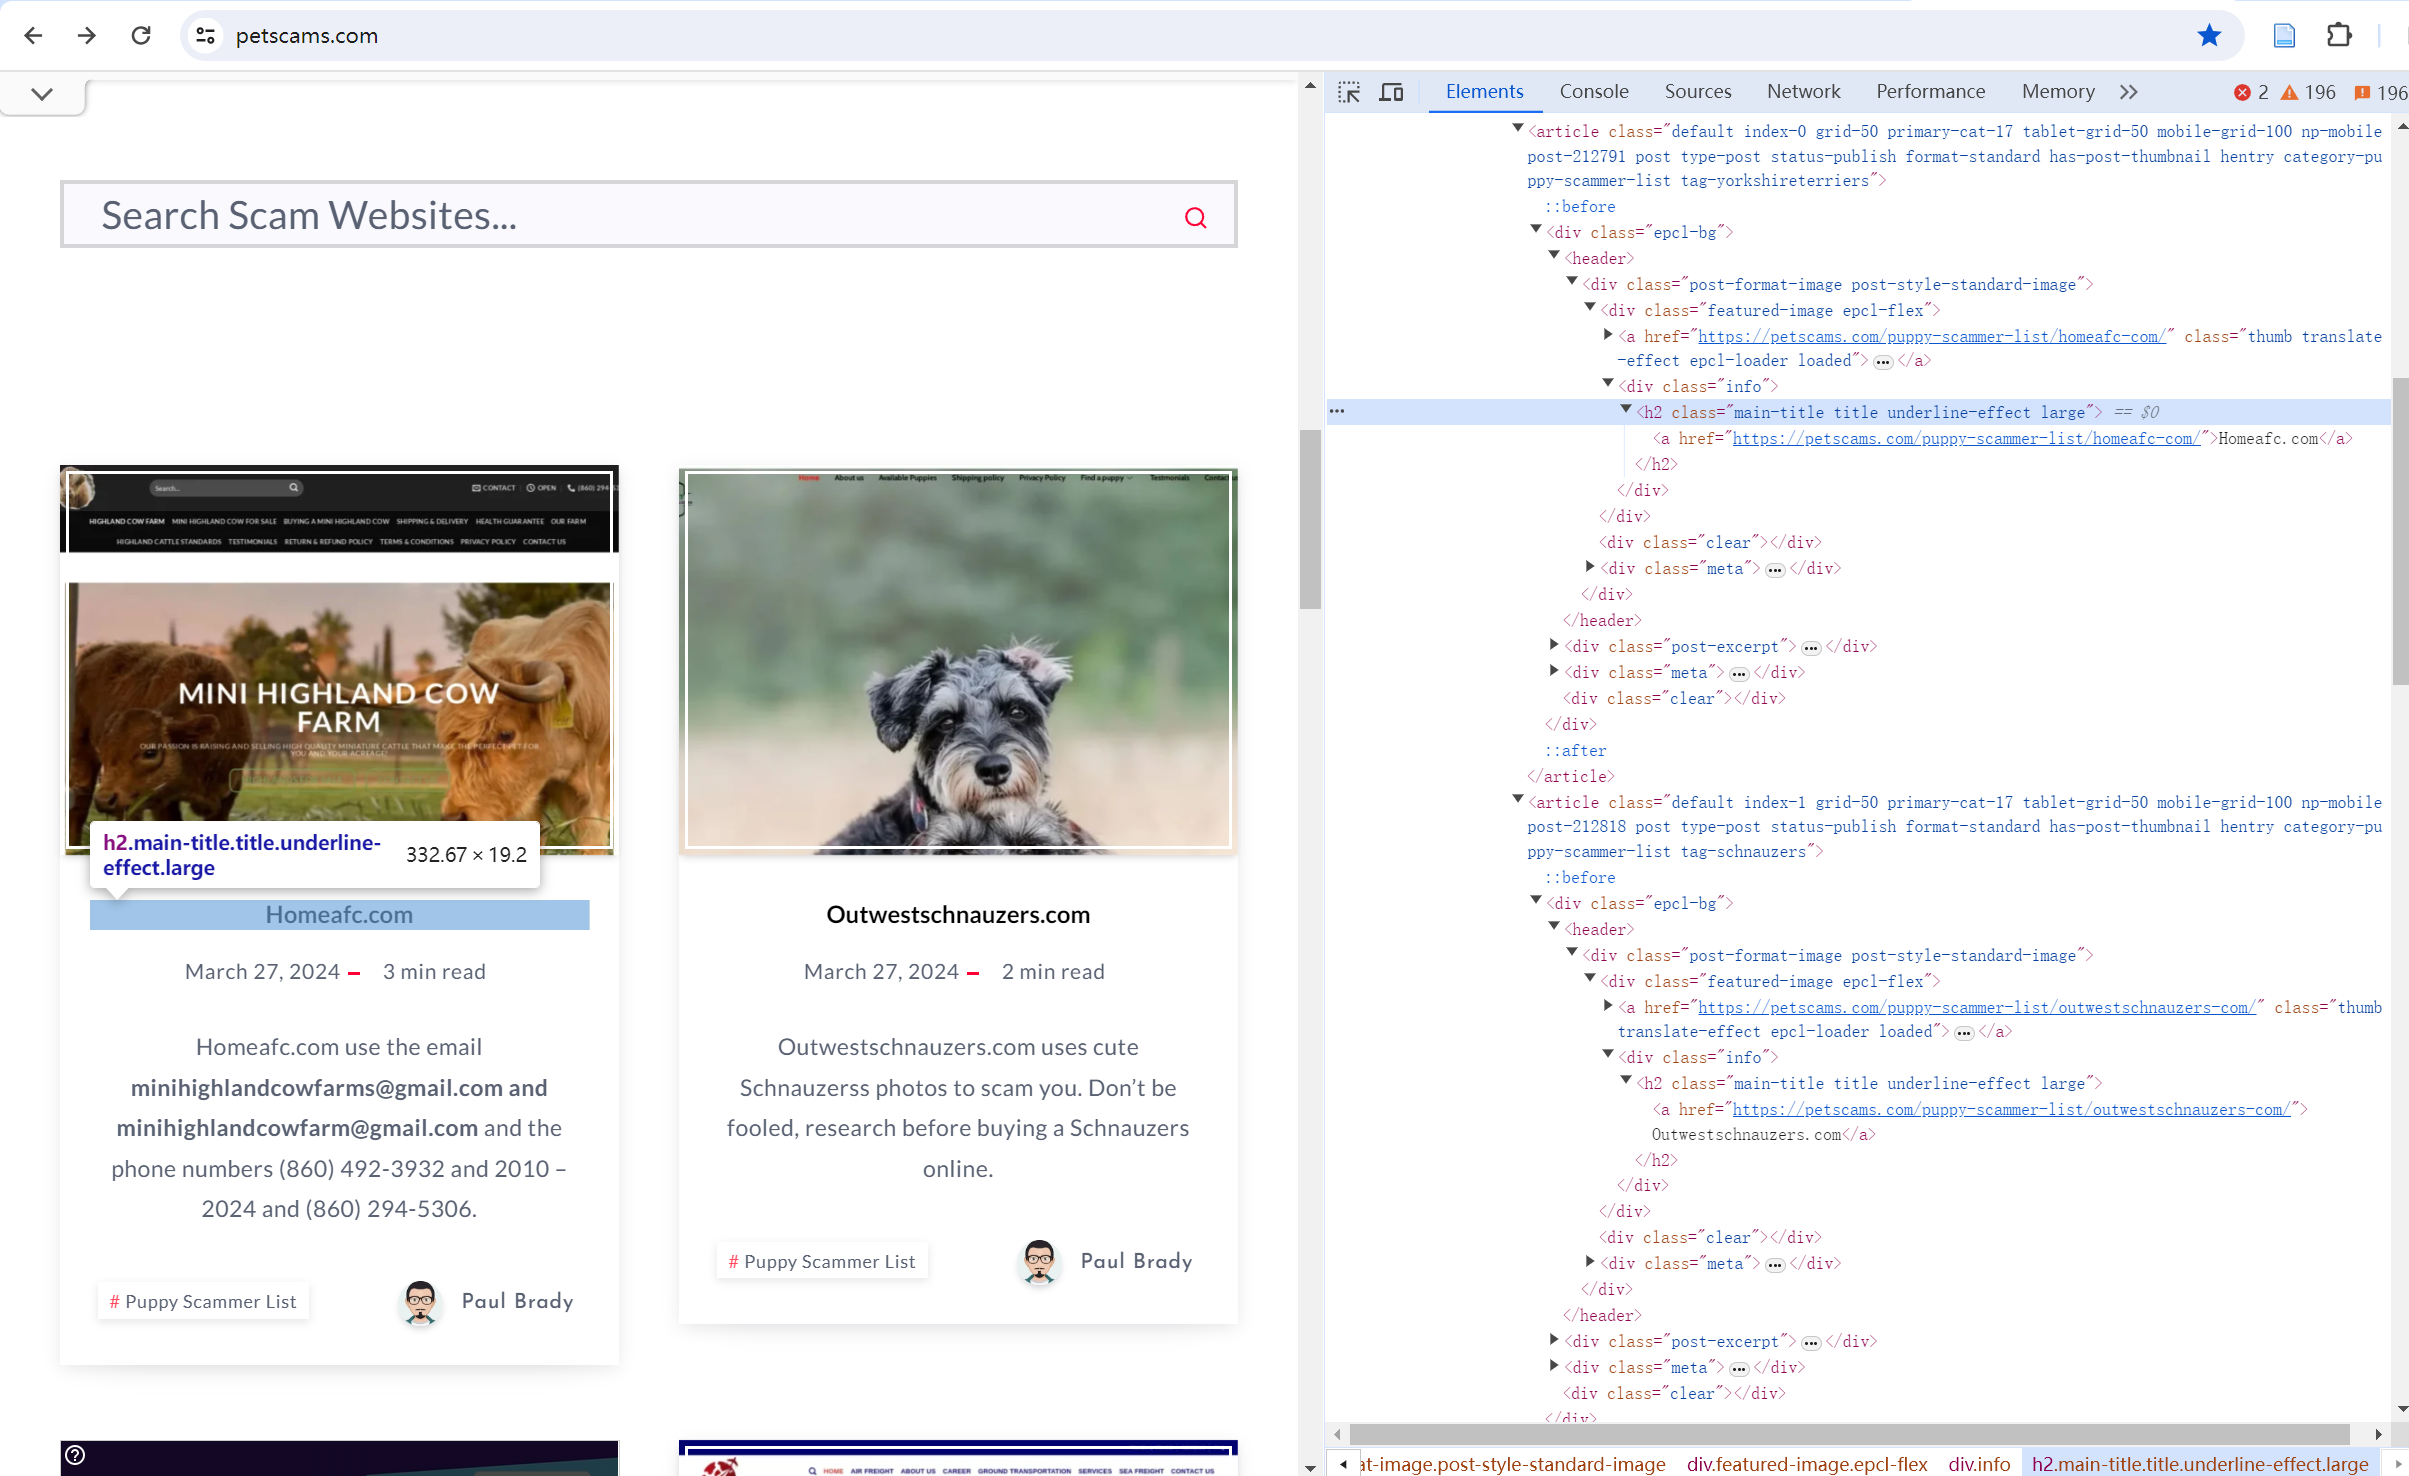
\includegraphics[width=\linewidth,height=0.28\textheight]{pic/figure1.png}
        \label{fig:petscams}
    \end{subfigure}
    \caption{Figure 1: Petscans.com in the developer mode}
    \label{fig:main1}
\end{figure}

\begin{figure}[!htb]\ContinuedFloat
    \centering
    % Second subfig
    \begin{subfigure}[b]{0.45\textwidth}
        
\includegraphics[width=\linewidth]{pic/figure2.png}
        \caption{Figure 2: Scam - Homeafc.com}
        \label{fig:sub2}
    \end{subfigure}
    \hfill % Used to add some space between subgraphs
    % Third subfig
    \begin{subfigure}[b]{0.45\textwidth}
        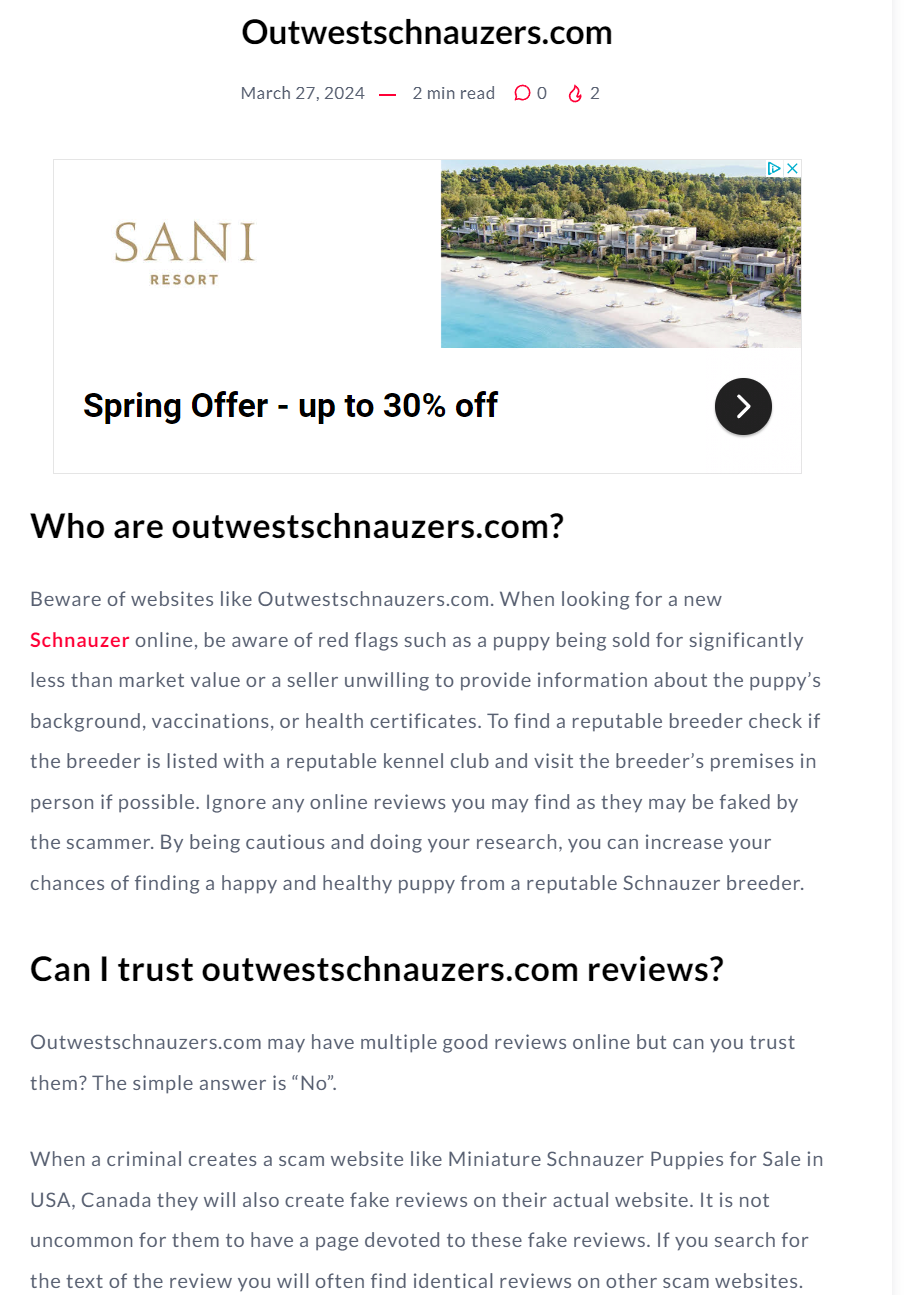
\includegraphics[width=\linewidth]{pic/figure3.png}
        \caption{Figure 3: Scam - Outwestschnauzers.com}
        \label{fig:sub3}
    \end{subfigure}
    \caption{Figure 2 (Homeafc.com) and Figure 3 (Homeafc.com)}
    \label{fig:main2}
\end{figure}

It is indicated that the function of ‘robots.txt’ is to tell search engines which URLs in the site are allowed for crawler access \cite{noauthor_robotstxt_nodate}. By visiting \url{https://petscams.com/robots.txt}, you can understand the scope of web crawling permissions set by the developers, and the text data returned in the page is as follows:
\vspace{10pt}

\noindent\hrule  
\begin{verbatim}
# START YOAST BLOCK
# ---------------------------
User-agent: *
Disallow:

Sitemap: https://petscams.com/sitemap_index.xml
# ---------------------------
# END YOAST BLOCK
\end{verbatim}
\hrule  
\vspace{10pt}


It can be seen that the configuration of the file is highly open. The rules specified by \href{https://www.petscams.com}{Petscams.com} permit all search engine crawlers to access all the content on the website, providing a solid foundation for the implementation of web scraping technologies.


\section{Web Scraping}
Compared to traditional manual data collection, web scraping can automatically retrieve unstructured data from a large amount of text such as HTML, then convert it into a structured format and store it locally \cite{khder_web_2021}. As Zhao stated \cite{zhao_web_2017}, the web scraping process mainly includes two parts: acquiring web resources and extracting specific information from the received data. The former refers to accessing the target webpage via the HTTP protocol, while the latter is to parse and extract the necessary data through automated scripts, and then save it in a specific format for further analysis. In this section, we will focus on discussing the most commonly used technology libraries when performing these two stages.
\\

In the first stage of web scraping, communication with the web server needs to be conducted through the HTTP, which is a request-response protocol that supports most web pages \cite{chandra_python_2015}. The Requests library in Python simplifies interaction with the target URL, providing efficient and reliable methods. As one of the most popular HTTP libraries, it supports the use of various HTTP methods, including GET, POST, PUT, and DELETE. Moreover, it also includes advanced features such as handling error and exception, authentication, redirects, sessions and SSL verification \cite{noauthor_requests_nodate}. These features meet all the requirements of the initial steps, ensuring the simplification of obtaining and processing server responses, including headers, session cookies, and status codes.
\\

For the second stage, various tech libraries can be utilised to parse and extract web data. Currently, BeautifulSoup, Selenium, and Scrapy are widely used because of their powerful capabilities. These tools focus on interactions with websites, as well as the extraction and parsing of data, each one demonstrating its own performance and advantages.
\\

BeautifulSoup is a Python library designed for parsing HTML and XML documents. It offers a simple and user-friendly syntax, enabling users to swiftly locate the necessary elements in the parsing tree using selectors like tag names, id names, etc \cite{chandra_python_2015}. For small or medium-sized crawling tasks on static web pages, BeautifulSoup can often be paired with the Requests library to form a lightweight crawling solution. It's important to note that this technology library primarily focuses on parsing work and does not involve constructing concurrent requests \cite{fariha_beautifulsoup_2023}.
\\

Similarly, Selenium does not support concurrent requests, which limits its efficiency in asynchronously executing multi-site scraping tasks to a certain extent. However, as a browser automation tool, Selenium supports multiple programming languages including Python, Java, and C\#, demonstrating unique capabilities in automating web browser operations \cite{fariha_beautifulsoup_2023}. Due to the unique support for JavaScript dynamically loaded pages \cite{fariha_beautifulsoup_2023}, it specialises in simulating human user actions, such as scrolling through pages, filling out forms, and clicking buttons. Additionally, unlike tools that need to be combined with the Requests library to send HTTP requests, scripts written by Selenium can run independently, using its built-in browser control functions to directly access and operate web pages. As the automated form filling will be introduced in project development, Selenium will become an indispensable tool library.
\\

Scrapy is a web crawler framework written in Python, which includes a complete set of web scraping solutions, including request handling mechanisms, data extraction, and database storage \cite{noauthor_intro_nodate}. Utilising the Twisted asynchronous network framework, Scrapy supports efficient concurrent request handling, making it particularly suitable for large-scale data crawling tasks and complex web data collection projects \cite{noauthor_intro_nodate}. Apart from being less self-sufficient in handling JavaScript than Selenium, and new users may encounter a certain learning curve, Scrapy better integrates the key functions of both Requests and BeautifulSoup. Thus, it can complete tasks independently in most scenarios without relying on external libraries.
\\

However, the demand of this project is relatively simple, there is no need to handle a large number of concurrent requests or complex data crawling. Therefore, I finally chose Requests, BeautifulSoup and Selenium as tools for the crawler development, since our main focus is to prioritise the smooth execution of the overall system process. While this approach may not be as comprehensive as Scrapy, it offers sufficient flexibility and convenience to meet project requirements. If necessary, it has also kept a door open for incorporating more efficient and complex crawling technologies in the future.


\section{Recognition and Processing of Text Data}
Throughout the construction and execution of the project system, various types of text data will be encountered, such as form content, email content, and time records. To manage these data effectively, this section introduces various methods for implementing information retrieval, guided by the heuristic search algorithm concept. These methods can be used separately or in combination, to ensure that the system identifies and processes text data accurately and efficiently.
\\

Heuristic search is a goal-oriented searching method. While it doesn't always guarantee the optimal solution, it usually provides high-quality solutions \cite{a_chapter_2001}. The heuristic search algorithm, also known as the A* algorithm, merges the benefits of keyword search and clustering. When dealing with NP problems that have incomplete solving conditions, the following evaluation function is established \cite{zhao_information_2014}:
\\

f(n)=g(n)+h(n)
\\

Here, f(n) represents the total estimated cost of node n, g(n) represents the actual path cost from the beginning state to node n, and h(n) stands for the heuristic estimated cost from node n to the goal. These values can help reflect the distance between the node and the goal, guiding the optimal path with each search step. This algorithm improves search efficiency by avoiding the exploration of invalid paths, thus improving the accuracy of vital information retrieval while ensuring the response speed. Therefore, the essence of heuristic search is to use limited information to achieve the search goal at the lowest cost. After acquiring substantial data through web scraping, this logic can also facilitate the fast batch retrieval of relevant information. Based on the characteristics or patterns of the data items, you can predefine the keyword groups, key data types, and different pattern matches. This allows scripts to execute "semi-structured" searches, effectively recognising and filtering vast amounts of text \cite{manning_introduction_2009}.
\\

Furthermore, the use of Regex and the FuzzyWuzzy library also demonstrates the application of heuristic search. As Uzum's report \cite{uzun_comparison_2018}, Regex is a sequence of characters that define a search pattern. With the introduction of the "re" module in Python, a pattern is predefined to extract data. However, this study also found that data extracted using Regex is only 43.5\% accurate compared to the expected data. Therefore, this project will consider using only simple Regex rules to remove unnecessary text information. 
\\

FuzzyWuzzy is a Python library used for string matching. Unlike Regex, once this library is utilised, a relevance score ranging from 0-100 need to be set \cite{majumder_fuzzywuzzy_2021}. The higher the score, the more closely the query word should match the target string. This can also be viewed as the retrieval constraints defined in retrieval heuristics \cite{yang_secure_2021}. By using fuzzy string matching, this heuristic method allows for a wider range of possibilities for a target string with uncertain content, thereby preventing over-matching a single query word.


\section{GPT Models}
In response to the demand for generating a large number of emails, the conventional approach involves using predefined text templates to generate email content. However, for a more advanced automated response system, I decided to integrate the GPT model.
\\

GPT, short for Generative Pre-Trained Transformer, has been extensively pre-trained on natural language data. It can predict and generate subsequent content after receiving text, images, or sound through the transformer \cite{3blue1brown_but_2024}. Since the release of the first GPT-1 version in June 2018, OpenAI has developed numerous models with various functions \cite{noauthor_openai_nodate}. For instance, the GPT series focuses on understanding and generating natural language or code; DALL·E specialises in image generation and editing; Whisper, a voice recognition model, and Jukebox is a music generation model. And these models are still being continuously updated and optimised.
\\

The core requirement of this project is to effectively understand and generate natural language text. In that case, the newly released GPT-3.5-turbo-0125 and GPT-4-0125-preview models both meet this requirement well. The processing capabilities of these two models have reached up to 60,000 tokens (approximately 45,000 English words) and 300,000 tokens (approximately 225,000 English words) per minute \cite{noauthor_openai_nodate}. This demonstrates that by integrating the API key into the system, adjusting both the necessary prompts and other parameters according to the code template provided by OpenAI \cite{noauthor_openai_nodate}, AI can automatically generate email content in batches using human language logic. Which will result in an efficient response speed and a natural interaction experience.




\chapter{Project Execution}
\section{Automatic Receipt of Inbound Emails}
Due to the large amount of email correspondence generated when the system induces fraudsters, the demand for the domain mail server has become a primary issue. In this project, two domains called “liveonline.ninja” and “malabaka.social” were registered on \href{https://www.name.com}{Name.com}, which were used for the system's testing and experimental stages in turn. \href{https://www.mailgun.com}{Maligun.com}, as a scalable email sending platform, is a significant tool for executing this project. Under the guidance of the official documentation \cite{noauthor_domain_nodate}, two domains were added in Mailgun and configured the DNS records to track the key information of all email correspondence under the domain.
\\

As shown in Figure 4, the Logs page of Mailgun allows users to view and track all email content and their statuses under the specified domain within the past five days of communications. However, these log records are automatically deleted after five days. To ensure the 31-days experiment can proceed smoothly, a script named \texttt{email\_crawl.py} was created for automated retrieval and long-term storage of inbound emails. First, configure the Mailgun API key and the required domain name in the system. Then, use the \texttt{request.get()} method to batch transfer emails based on a customised time range and event status. Each email should be named according to its unique receiving time, represented by the Unix timestamp. To ensure readability of the archived email content, the program formats each inbound email by retaining only the title, body, sender, and recipient information. This information is finally stored in a separate JSON file.
\begin{figure}[!htb]
    \centering
    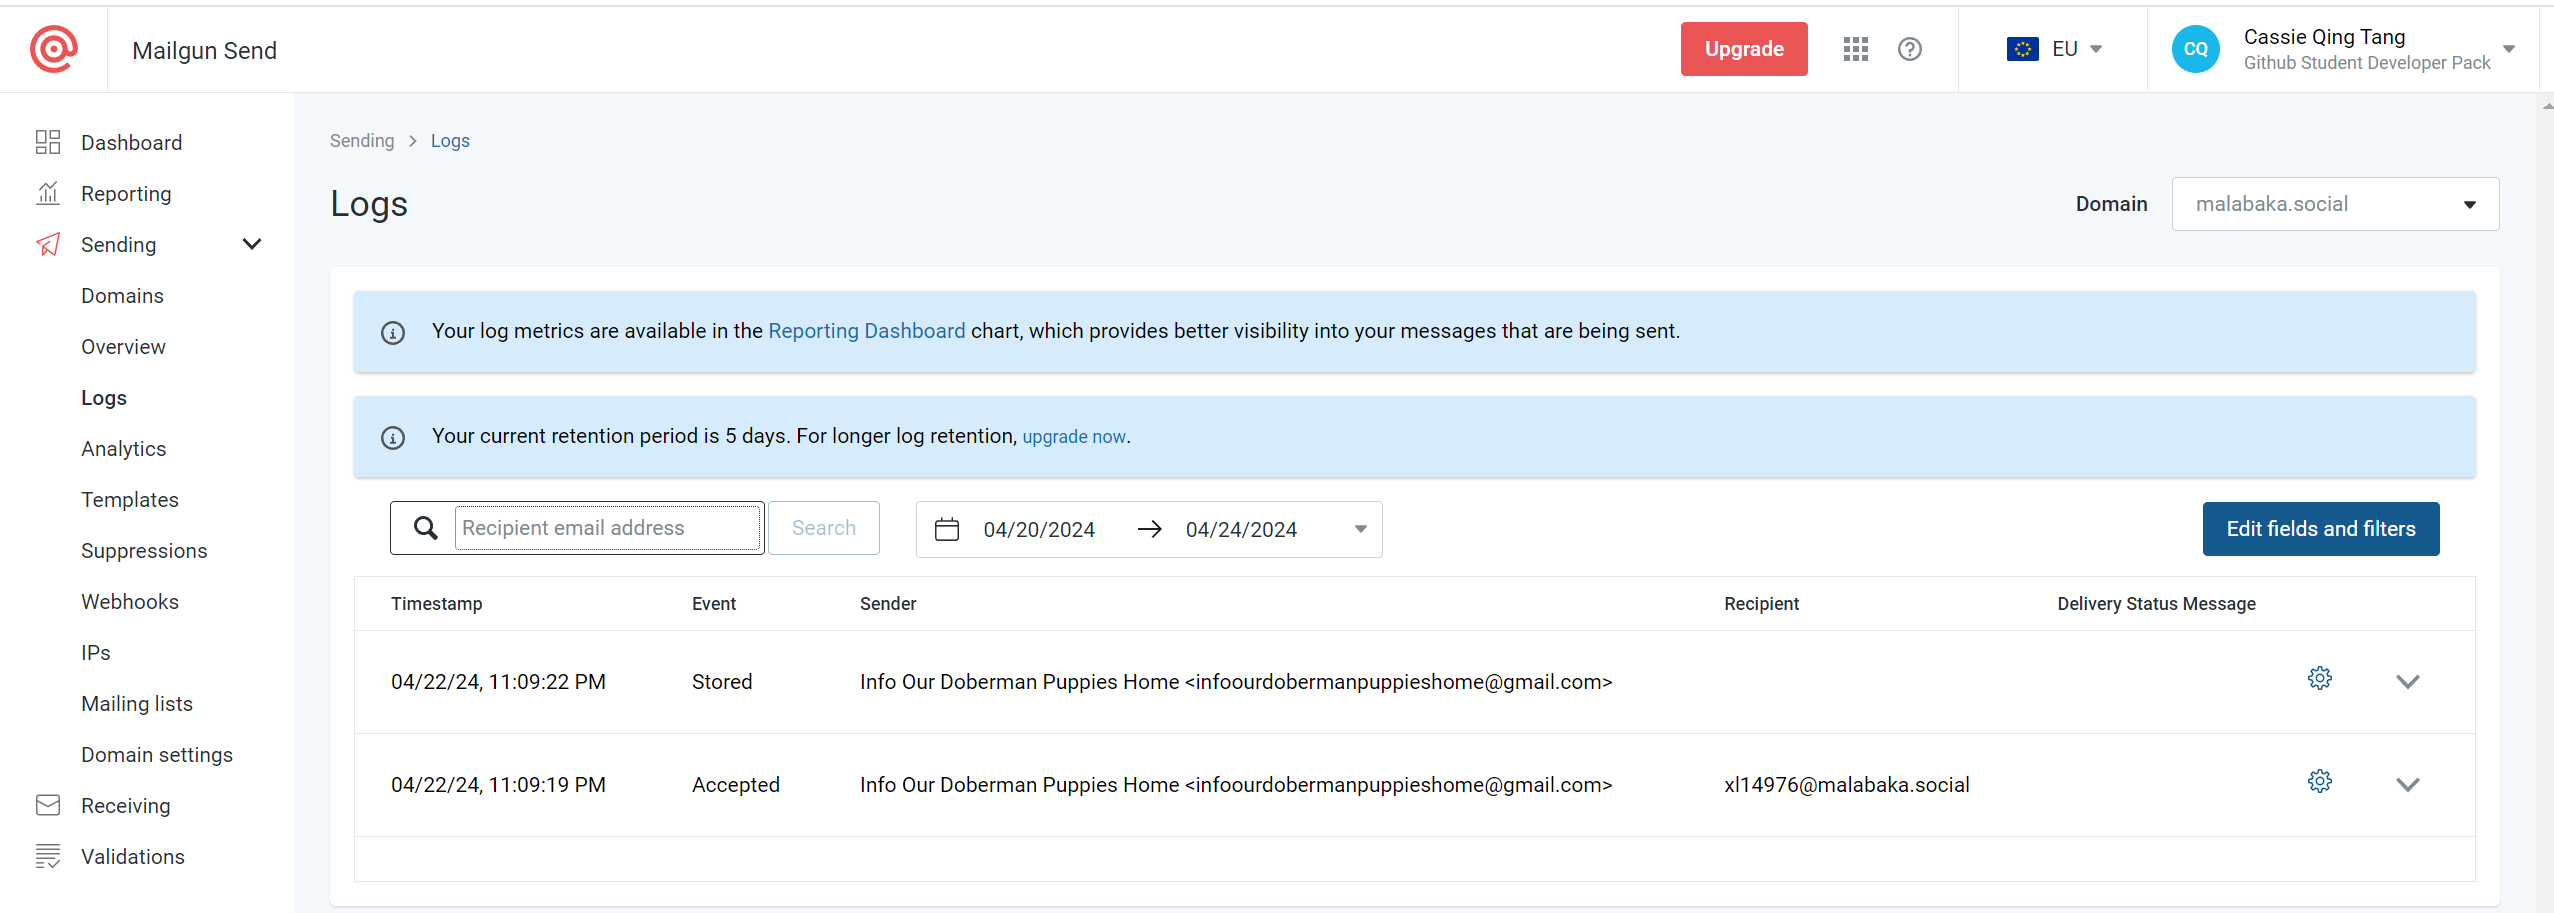
\includegraphics[width=0.85\linewidth,height=0.2\textheight]{pic/figure4.png}
    \caption{Figure 4: Mailgun logs page of malabaka.social}
\end{figure}


\section{Implementation of Web Scraping}
In this project, web scraping is primarily used to access, collect, and fill in a large amount of data on the form pages of pet scam websites. We have learned before that \url{www.petscams.com} is a key resource, dedicated to collecting and reporting information on scam websites related to pet sales and transportation. Given that pet transportation scams are often only involved in the later stages of scam activities, and these scam websites do not expect consumers to contact them proactively. Therefore, our crawlers will only focus on those fraudulent pet websites involved in sales.

\subsection{Crawling and Filtering List of Target Websites}
The scraping process begins with \texttt{petscam\_crawl.py}, which targets fake pet sales websites on \url{https://petscams.com/category/puppy-scammer-list/}. It fetches HTML pages using the requests library and parses them with BeautifulSoup using 'html.parser'. The script identifies each $<$article$>$ tag, then uses the $<$time$>$ and $<$h2 class="main-title"$>$ tags within to filter articles by publication date and extract scam domain names.  Each extracted domain is automatically prefixed with 'https://' to ensure they are directly accessible.
\\

While randomly visiting some of the URLs reported in recent months, it was found that some of them have already expired or been suspended. This issue is more prevalent with scam domain names revealed earlier. As a result, the code includes checks for the return status code of the link and potential message prompts such as "Account Suspended" and "Maintenance mode is on". On the other hand, the administrators of \url{petscams.com} occasionally re-post the same websites, which can lead to duplicate links saved in the JSON list. Taking advantage of the characteristic that sets do not allow duplicate elements \cite{sturtz_sets_nodate}, all valid URLs are first stored in a set, then converted into a list format and stored in a JSON file. These strategies can effectively prevent the potential waste of time and decrease in accuracy that invalid or duplicate links could cause in the subsequent code execution process.
\\

Next, heuristic search will be used to retrieve the contact form pages that exist in the website list collected in the previous step, which is done by a crawler program called \texttt{contactpage\_crawl.py}. Based on observations of a large number of pet scam sites, scammers usually set up a "Contact Us" page, guide people to leave their contact information, and thus get in touch with the victims separately. Through Chrome's developer mode, I summarised the three common structures they often use when developing this page, and wrote the code according to them.
\\

Some scam websites place the contact form directly on the main page instead of setting up a separate submission page. Since $<$form$>$ element is frequently used to initiate and nest form content \cite{noauthor_how_2024}, the script first checks for the existence of $<$form$>$ and common elements within it, like $<$input type = "email"$>$, on the main page. If these exist, the main page's URL is directly used as the target form page URL and stored in a JSON file. If these elements are not found on the homepage, the script continues to search for links containing specific keywords, such as "contact-us" or "reach-us". The form links related to these keywords are usually found in the $<$a href$>$ tag. Moreover, some scammers choose to put the form URL contained in the $<$a href$>$ tag in the $<$li$>$ tag instead of $<$form$>$. Thus, the code also includes keyword retrieval for this potential structure.

\subsection{Automated Form-Filling}



\section{Implementation of Email Automation Responses}

\subsection{Integrating Response Strategies}





\section{Construction and Operation of the System}
The system was built on an open-source, expandable scam-baiting mail server \cite{an19352_an19352scambaiter_back_2023}, which means that there is no need to construct a basic architecture from scratch. As a result, the simplified development process involves adding own crawlers, customising the reply procedure for pet scammers, and configuring API keys and data storage directories.




\chapter{Analysis of results}



\chapter{Critical Evaluation}









\chapter{Conclusion}
In conclusion, this project effectively combats the rise of online pet scams by employing an automated system designed to deplete scammers' resources and deter fraudulent activities. Over a four-week experimental phase, four robotic responders consistently engaged scammers, wasting at least a month of their time. Dozens of scammers continued to interact with the system even after the experiment concluded. This not only aids in scam prevention but also refines scam-baiting strategies, contributing valuable insights into the fight against non-delivery fraud and advance fee fraud.
\\

Besides, the future direction of this project may focus on integrating the script for filling non-delivery fraud websites with other systems that can classify fraudulent advertisements or websites. This could include the code for automatic detection of pet scam websites \cite{mehmedov_automated_2021}.



% \bibliographystyle{ieee}
\bibliography{references}

\appendix

\chapter{Appendix A: }
\label{}






\end{document}
